\documentclass[11pt,a4paper]{article}
\usepackage{fontspec}
\setmainfont{TeX Gyre Pagella}
\newfontfamily\headfont{Inter}[UprightFont=*-ExtraBold,BoldFont=*-ExtraBold,Extension=.otf,Path=/usr/share/fonts/opentype/inter/]
\usepackage[a4paper,margin=2.3cm]{geometry}
\usepackage{graphicx,booktabs,float,caption,array,xcolor,longtable}
\usepackage{xurl}
\usepackage[hidelinks]{hyperref}
\usepackage{titlesec}
\usepackage[round]{natbib}
\usepackage{setspace}
\setstretch{1.05}
\renewcommand{\topfraction}{0.9}
\renewcommand{\bottomfraction}{0.8}
\renewcommand{\textfraction}{0.1}
\renewcommand{\floatpagefraction}{0.75}
\setlength{\parindent}{0pt}
\setlength{\parskip}{0.55em}
\titleformat{\section}{\headfont\Large}{\thesection}{0.8em}{}
\titleformat{\subsection}{\headfont\large}{\thesubsection}{0.8em}{}
\captionsetup{font=small,labelfont=bf}
\urlstyle{same}
\hypersetup{pdftitle={Painted Places},pdfauthor={Tristan Hotham}}

\begin{document}
\begin{center}
{\Large\bfseries Painted Places\par}
\vspace{0.4em}
{\large Where catalogued landscape, marine and city paintings look, and how far painters went from home:\\8,533 paintings and 4,740 depicted places in Wikidata\par}
\vspace{1.2em}
{\large Tristan Hotham\par}
\vspace{0.3em}
{\small Independent researcher\\
ORCID: 0000-0003-4931-9349\\
DOI: https://doi.org/10.5281/zenodo.23873007\par}
\vspace{0.8em}
2026
\end{center}

\begin{center}\textbf{Abstract}\end{center}
I map every painting in Wikidata that is classed as a landscape, marine painting or cityscape and that depicts an item with coordinates, after removing depicted items that are not places on the Earth (events such as sea battles, ships, and the Moon, whose coordinates lie on the lunar globe). The result is 8,533 paintings by 2,393 named painters showing 4,740 places in 102 countries. The most painted place is the Seine (228 paintings by 81 painters), followed by Paris, Lofoten, Venice and Nordland. Linking painters' birthplaces gives a distance for 7,183 paintings: the median is 231 km, 26\% lie within 50 km of the birthplace and 26\% more than 1,000 km away. Distances rise from a median of 48 km in the 1600s to 331 km in the 1800s, and the geography shifts from the Netherlands (62\% of 1600s paintings) to Italy (37\% in the 1700s) to France (27\% in the 1800s). Coverage is uneven: the largest collection holds 6.6\% of the paintings, 39\% of them by a single painter, the ten largest 30\%, and 80\% of paintings show places in Europe. The map describes what has been catalogued as much as where painters went.

\textbf{Keywords:} landscape painting; Wikidata; cultural heritage data; art geography; painters' travel; museum collections; open data

\section{Introduction}
Landscape painting is about places, and many of its places are famous in their own right: Monet's Seine, Canaletto's Venice and London, the Hudson River School's Catskills. Art historians have studied painters' travels one artist or one school at a time. Linked open data now make it possible to look at many painters at once. Wikidata records, for hundreds of thousands of paintings, a creator, a date, a collection, a genre and, increasingly, what the painting depicts. When the depicted item is a river, a town or a mountain it carries coordinates. This paper uses those statements to map where catalogued landscape, marine and city paintings look, which places painters returned to, how far from their birthplaces they painted, and how the geography changed over four centuries. Because the source is a catalogue assembled by museums, projects and volunteers, the paper also measures how far a few contributors shape the result.

\section{Data}
I queried Wikidata \citep{wikidata} through the QLever SPARQL endpoint \citep{qlever} on 1 November 2026 for items that are instances of painting, have a genre of landscape art, marine art or cityscape (or of three related genres, religious art, genre painting and animal painting) and depict an item with coordinates, together with the creator, inception date, image, collection and number of Wikipedia articles. The query returned 18,249 rows for 10,321 paintings. A second query returned each creator's country of citizenship and the coordinates of the place of birth, and a third the 2 paintings with a separate ``coordinates of depicted place'' statement. Natural Earth \citep{naturalearth} provides countries (today's borders), first level regions and continents.

\section{Methods}
\subsection{Paintings and places}
I keep the 8,757 paintings with at least one of the three landscape genres and set aside 1,564 that entered only through a related genre. The ``depicts'' property catches anything with coordinates, so I remove depicted items that are not places. The rule, applied in order, is: the coordinate must be a point on the Earth (this removes 3 items, chiefly the Moon, which appears in 138 paintings); the coordinates must be in range and not 0,0; and the item must not be an event (70 items, mostly naval battles), a vessel (19) or another non-place (2). The non-places are listed by identifier in the code after reading every depicted item with two or more paintings and a keyword scan of all labels; the build fails if the scan finds an unlisted event or ship. 224 paintings lose all their places and are dropped, leaving 8,533 paintings, 4,740 places and 11,176 painting and place pairs. Table~\ref{tab:excluded} lists the most frequent exclusions.

\begin{table}[tbp]\centering\small\caption{The depicted items most often removed as not being places (painting and item pairs).}\label{tab:excluded}\begin{tabular}{p{6cm}p{6cm}r}\toprule Item & Reason & Pairs\\\midrule
Moon & not a point on the Earth (another globe or an unknown value) & 138\\
HMS Prince Royal & vessel & 7\\
Four Days' Battle & event & 6\\
Bombardment of Algiers & event & 5\\
Battle of Solebay & event & 5\\
Battle of Texel & event & 5\\
Spanish Armada & event & 4\\
Battles of Barfleur and La Hougue & event & 4\\
Titanic & vessel & 3\\
Raid on the Medway & event & 3\\
\bottomrule\end{tabular}\end{table}

\subsection{Distances, periods and kinds of place}
For each painting with a painter whose birthplace has coordinates, I compute the great circle distance from the birthplace to each depicted place and take the median across places. Broad areas (countries, first level regions, seas and oceans; 156 places) are excluded from distances when a painting also names a finer place, and paintings that name only broad areas are left out. Rivers are single points in Wikidata, so distances to rivers are approximate. Periods group inception years by hundreds (the 1800s are 1800 to 1899); paintings before 1600 are grouped together and the few after 1999 join the 1900s. Country shares split a painting equally between its places. The 100 most painted places were assigned by hand to six kinds (rivers and canals; cities, towns and villages; coasts, seas and islands; mountains, valleys and forests; buildings, bridges and squares; regions and countries).

\section{Results}
\subsection{The most painted places}
Figure~\ref{fig:map} maps all places and Figure~\ref{fig:europe} shows western Europe. The Seine is the most painted place, with 228 paintings by 81 painters; Monet (38), Sisley (27) and Pissarro (15) together account for 35\% (Figure~\ref{fig:top}, Table~\ref{tab:places}). Among the 100 most painted places, 30 are cities, towns or villages, 20 buildings, bridges or squares, 16 rivers or canals, 13 coasts, seas or islands, 13 mountains, valleys or forests and 8 regions or countries; 8 of the top 25 are rivers, coasts or seas. The distribution has a long tail: 68\% of places appear in only one painting and 155 in ten or more.

\begin{figure}[tbp]\centering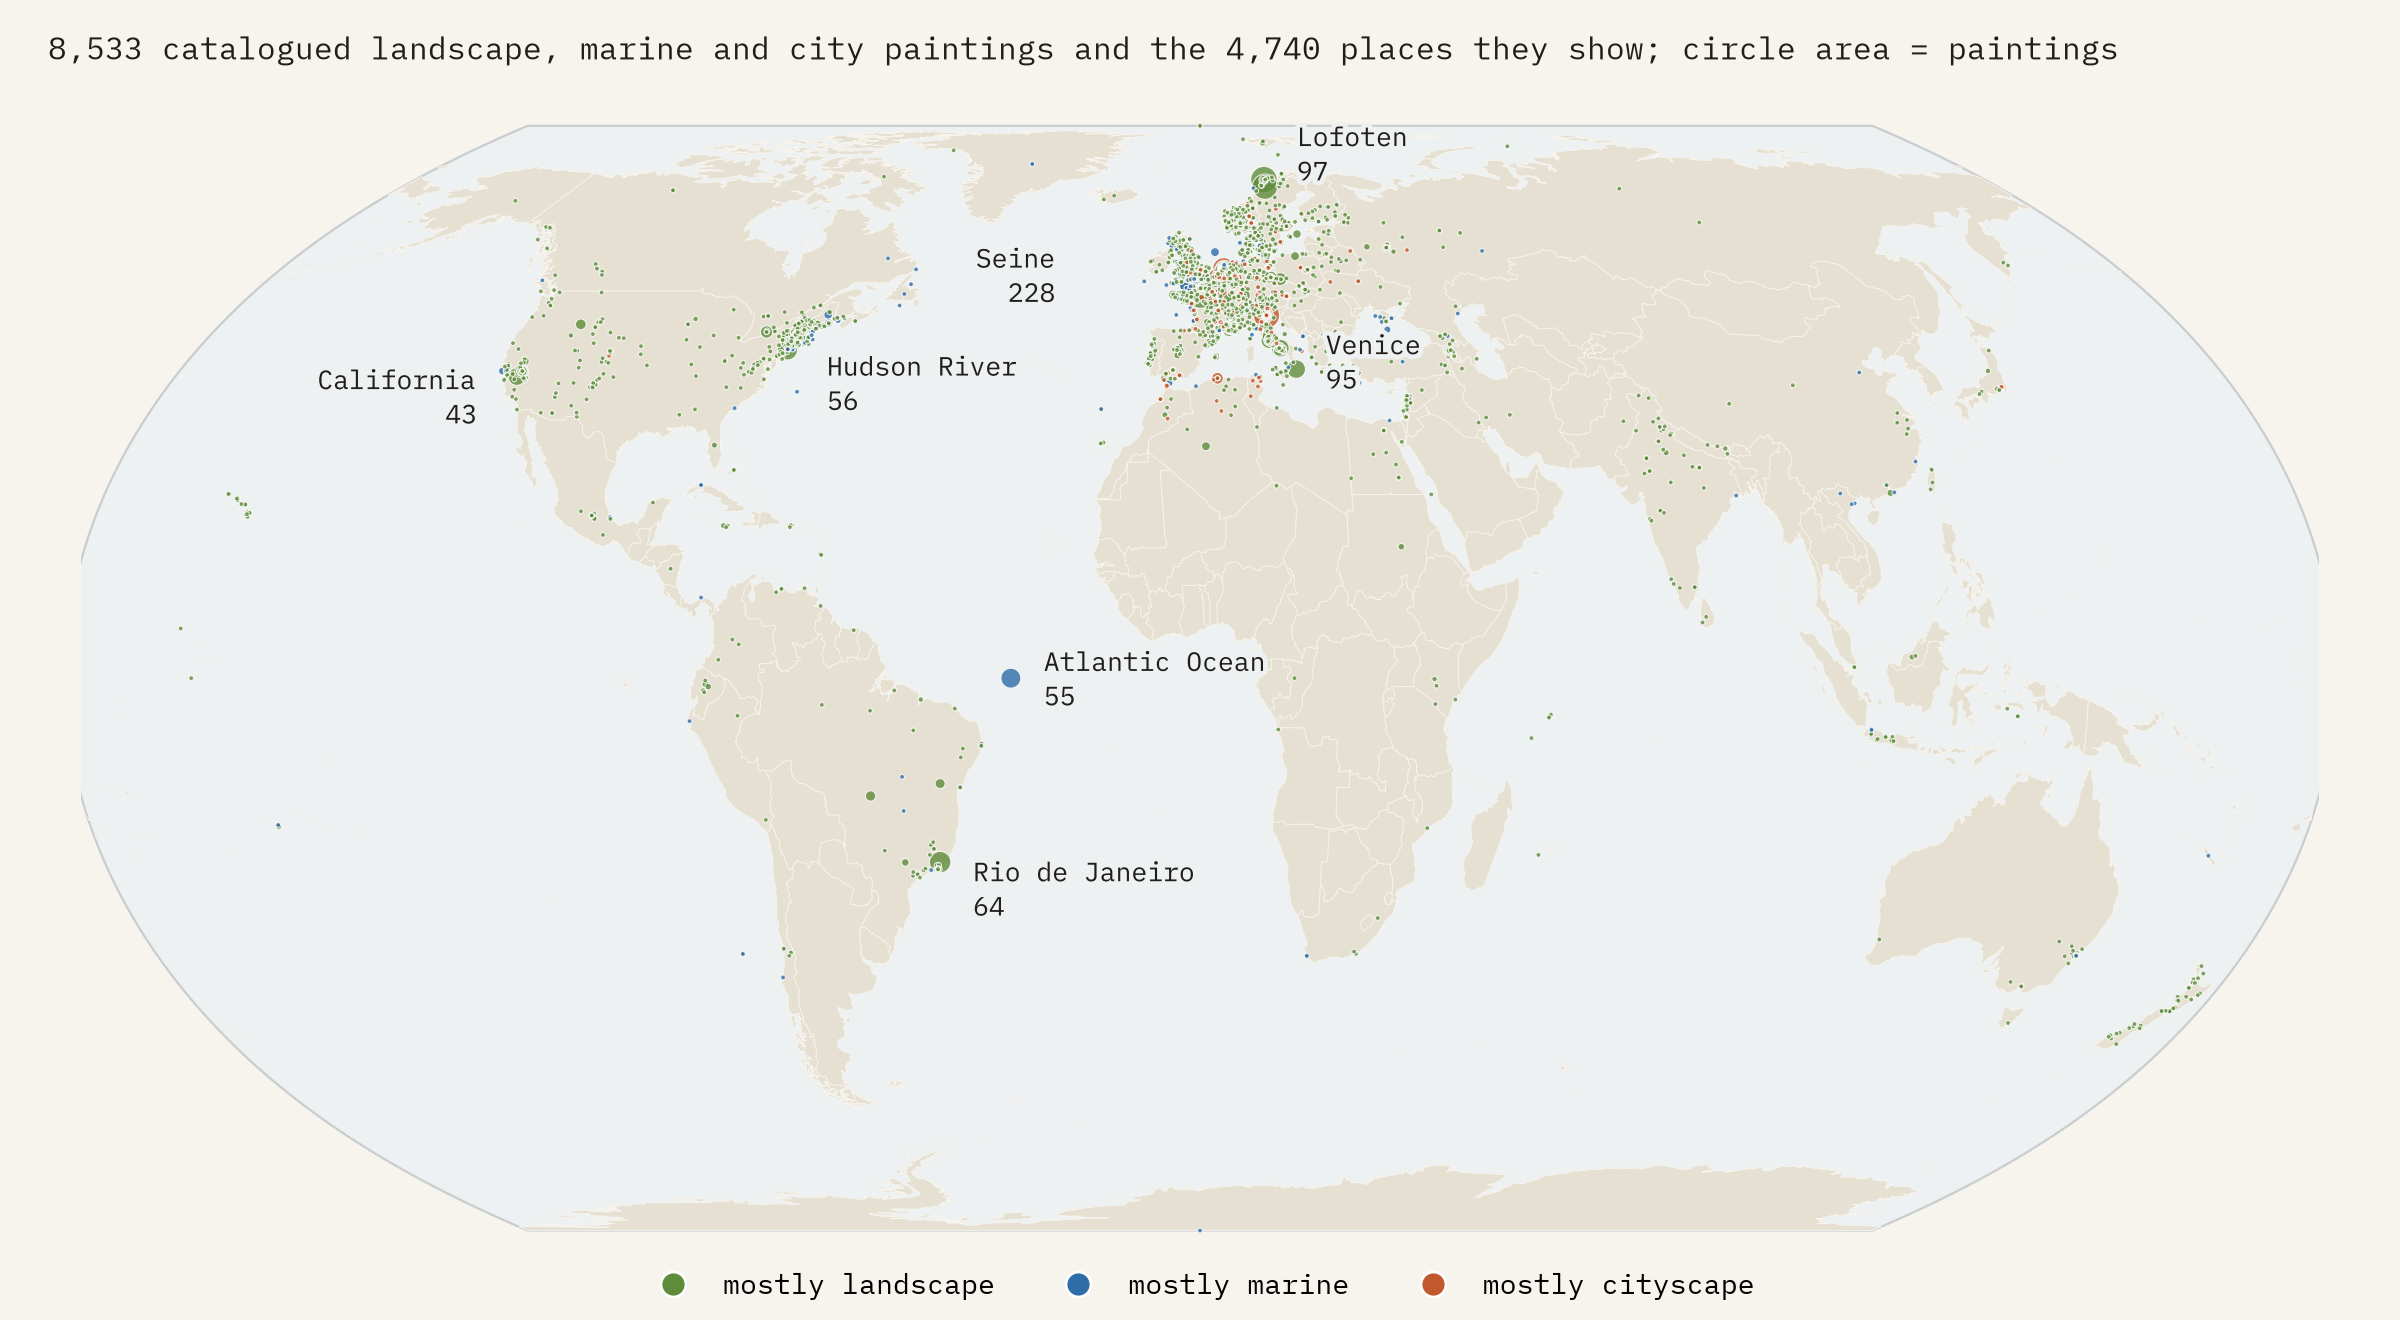
\includegraphics[width=\textwidth]{f_map.png}\caption{All 4,740 depicted places, sized by the number of paintings and coloured by the dominant genre.}\label{fig:map}\end{figure}
\begin{figure}[tbp]\centering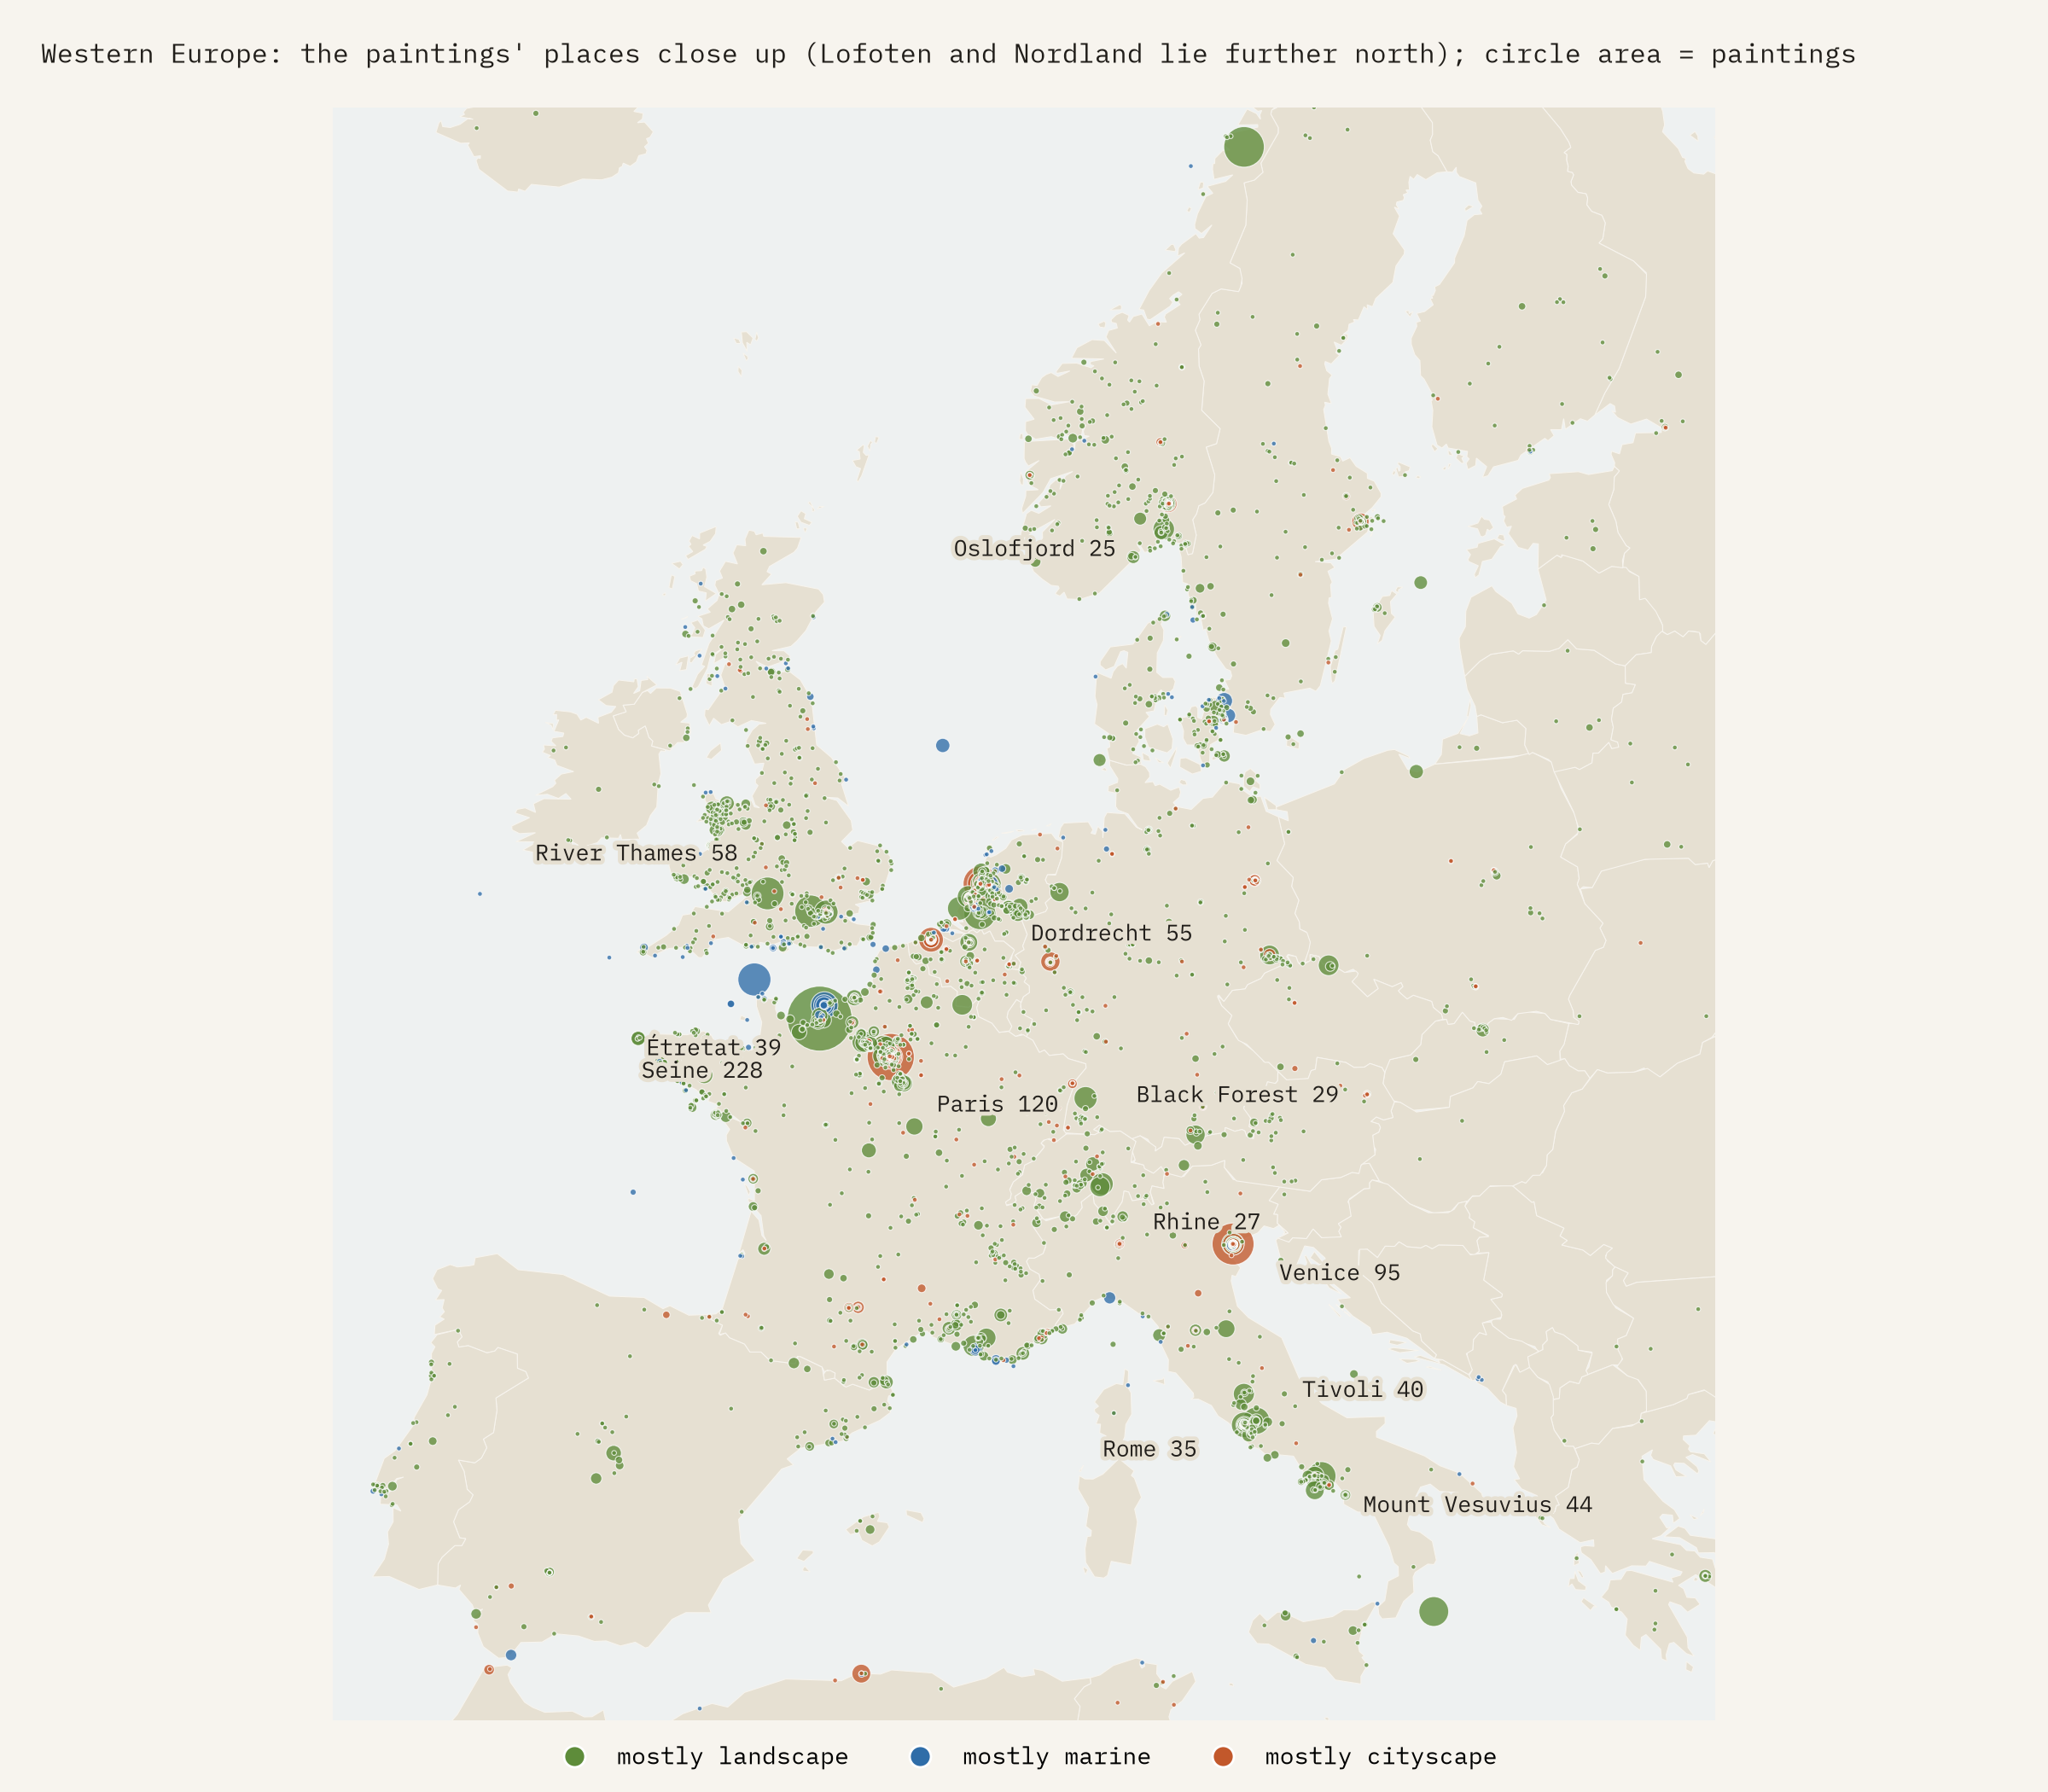
\includegraphics[width=.92\textwidth]{f_europe.png}\caption{Western Europe in detail (European equal area projection).}\label{fig:europe}\end{figure}
\begin{figure}[tbp]\centering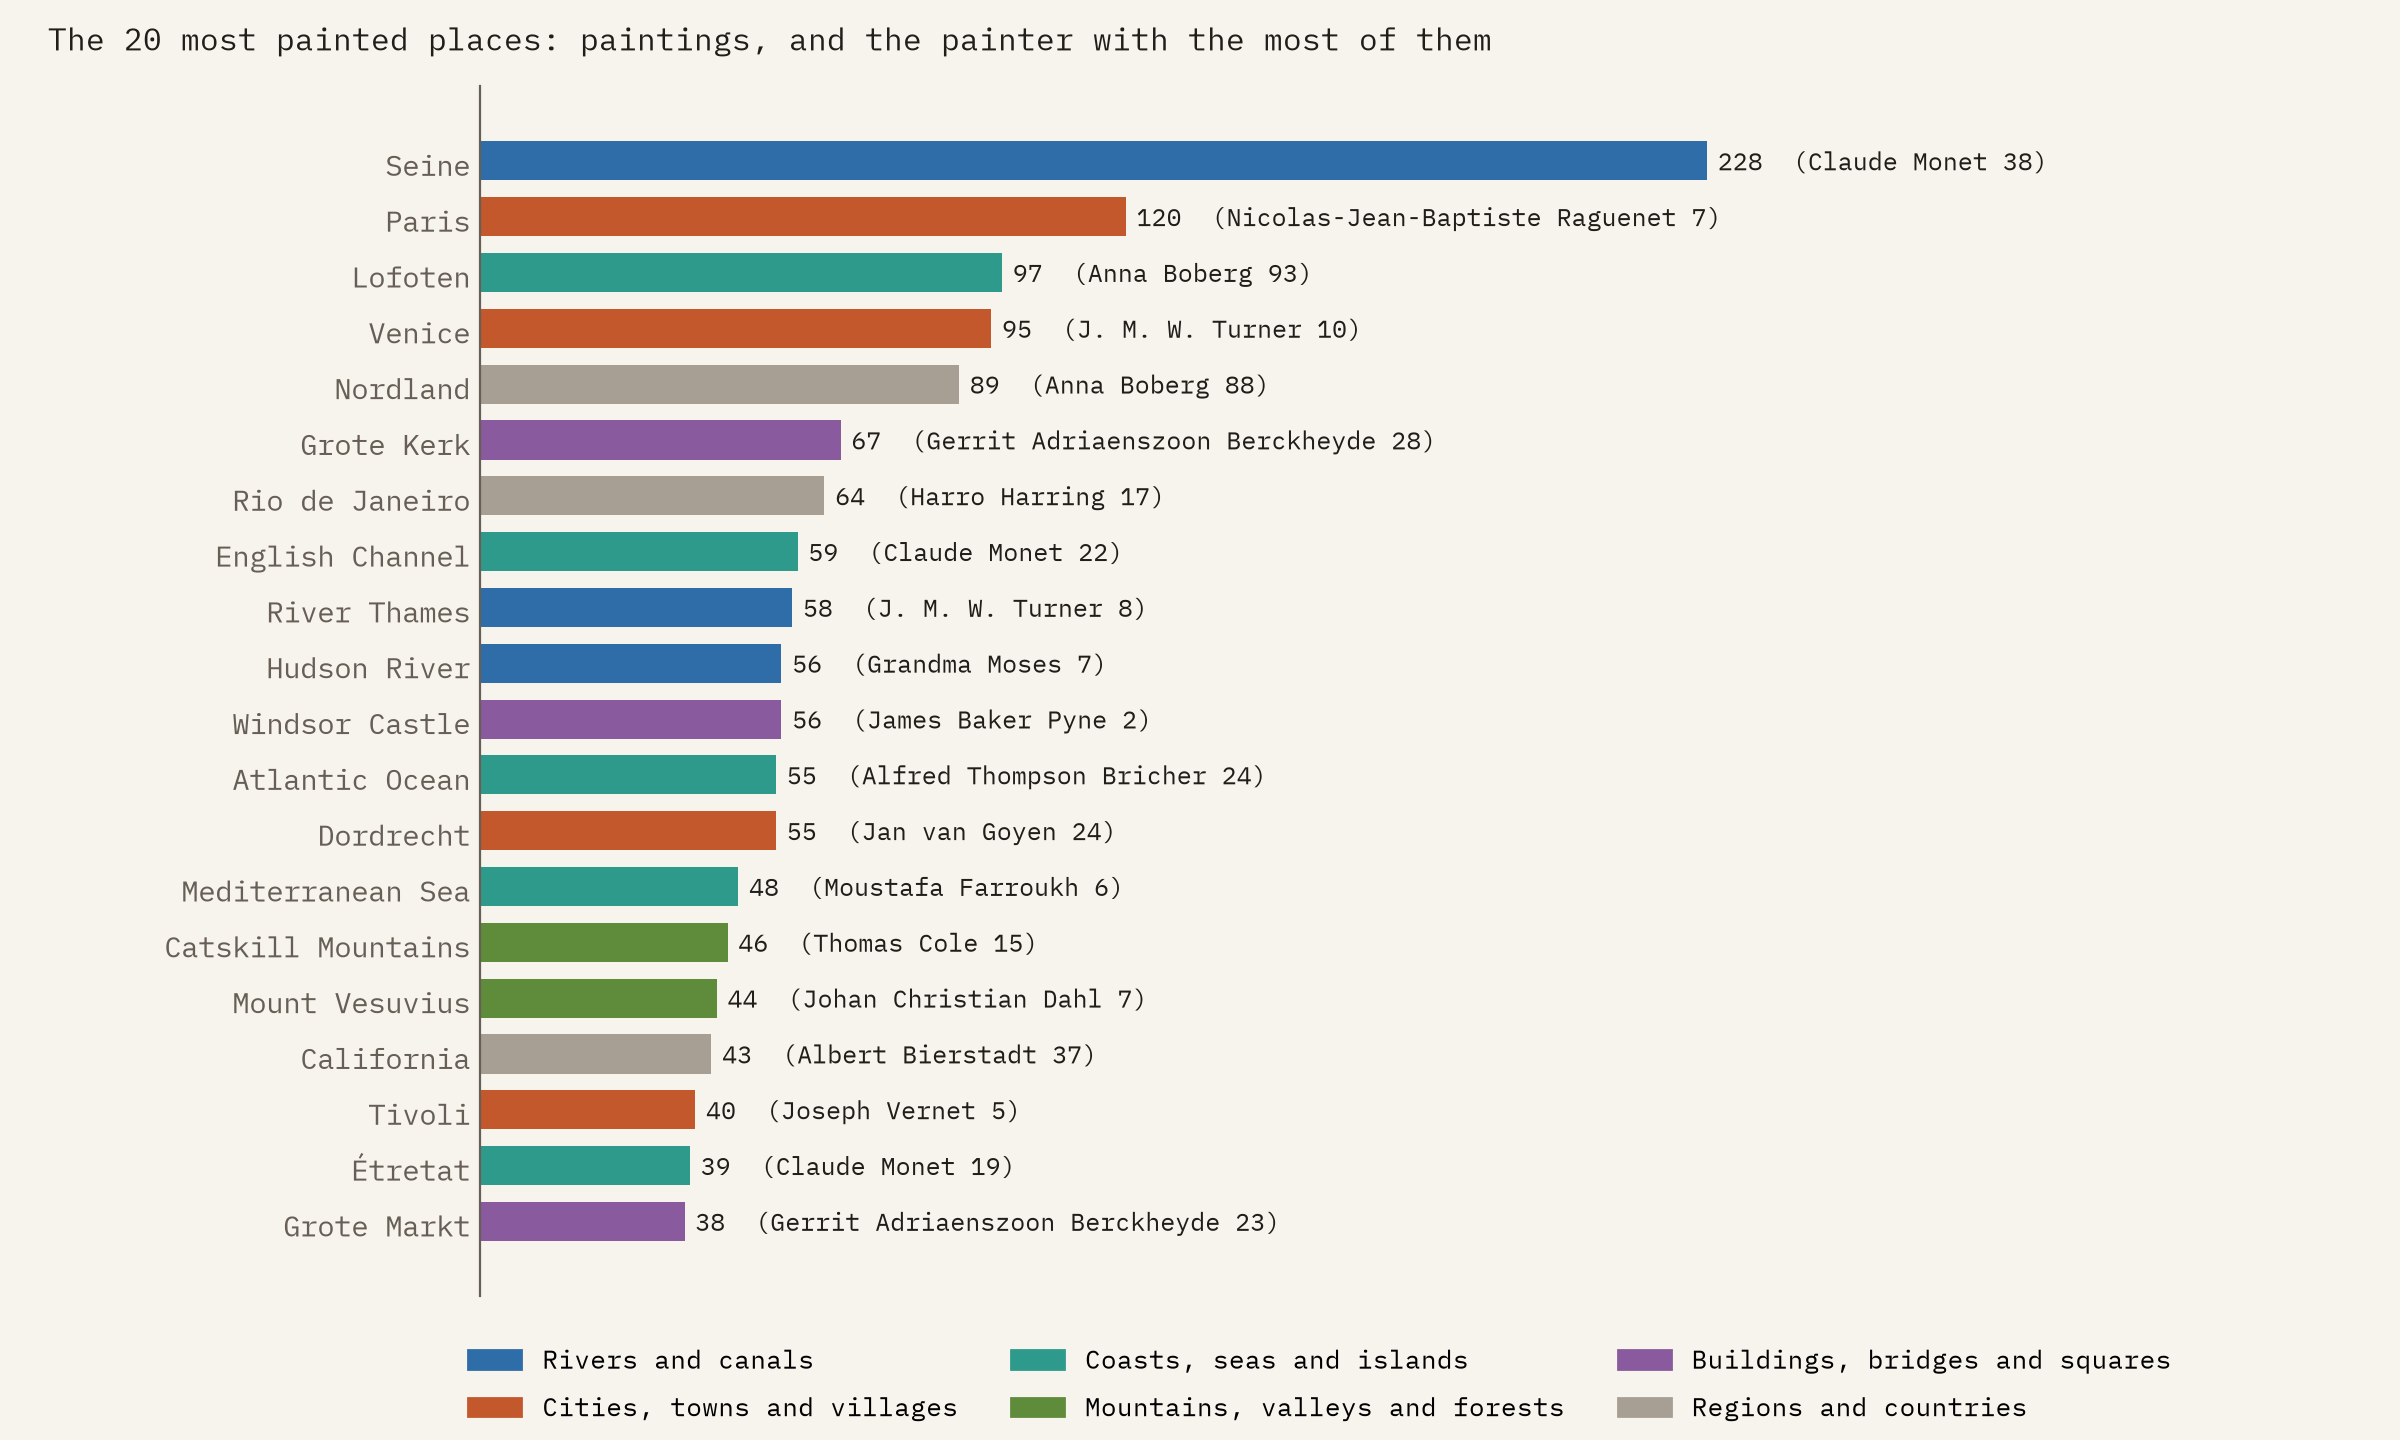
\includegraphics[width=\textwidth]{f_top.png}\caption{The 20 most painted places, coloured by kind, with the painter who painted each most often.}\label{fig:top}\end{figure}

\begin{table}[tbp]\centering\footnotesize\setlength{\tabcolsep}{4pt}\caption{The 25 most painted places: paintings, painters, and the leading painter and collection.}\label{tab:places}\begin{tabular}{p{2.9cm}p{2cm}rrp{3.5cm}p{3.6cm}}\toprule Place & Country & Paintings & Painters & Leading painter & Leading collection\\\midrule
Seine & France & 228 & 81 & Claude Monet (38) & Musée d'Orsay (73)\\
Paris & France & 120 & 76 & Nicolas-Jean-Baptiste Raguenet (7) & Musée d'Orsay (34)\\
Lofoten & Norway & 97 & 5 & Anna Boberg (93) & Nationalmuseum (93)\\
Venice & Italy & 95 & 50 & J. M. W. Turner (10) & Musée d'Orsay (11)\\
Nordland & Norway & 89 & 2 & Anna Boberg (88) & Nationalmuseum (89)\\
Grote Kerk & Netherlands & 67 & 24 & Gerrit Adriaenszoon Berckheyde (28) & Frans Hals Museum (11)\\
Rio de Janeiro & Brazil & 64 & 19 & Harro Harring (17) & Brasiliana Iconográfica (64)\\
English Channel & France & 59 & 23 & Claude Monet (22) & Musée d'Orsay (13)\\
River Thames & United Kingdom & 58 & 30 & J. M. W. Turner (8) & National Trust (10)\\
Hudson River & United States & 56 & 26 & Grandma Moses (7) & Brooklyn Museum (6)\\
Windsor Castle & United Kingdom & 56 & 27 & James Baker Pyne (2) & National Trust (50)\\
Atlantic Ocean & at sea & 55 & 21 & Alfred Thompson Bricher (24) & Metropolitan Museum of Art (5)\\
Dordrecht & Netherlands & 55 & 14 & Jan van Goyen (24) & Dordrechts Museum (4)\\
Mediterranean Sea & at sea & 48 & 24 & Moustafa Farroukh (6) & Sursock Museum (5)\\
Catskill Mountains & United States & 46 & 14 & Thomas Cole (15) & Metropolitan Museum of Art (3)\\
Mount Vesuvius & Italy & 44 & 28 & Johan Christian Dahl (7) & Condé Museum (9)\\
California & United States & 43 & 6 & Albert Bierstadt (37) & Fine Arts Museums of San Francisco (4)\\
Tivoli & Italy & 40 & 30 & Joseph Vernet (5) & Musée Fabre (6)\\
Étretat & France & 39 & 11 & Claude Monet (19) & Musée d'Orsay (5)\\
Grote Markt & Netherlands & 38 & 12 & Gerrit Adriaenszoon Berckheyde (23) & Frans Hals Museum (11)\\
Amsterdam & Netherlands & 36 & 17 & Ludolf Bakhuizen (7) & Department of Paintings of the Louvre (4)\\
Rome & Italy & 35 & 25 & François Marius Granet (3) & National Trust (4)\\
Pont Neuf & France & 33 & 16 & Camille Pissarro (5) & Musée Carnavalet (15)\\
Bruges & Belgium & 33 & 22 & Jan Baptist van Meunincxhove (2) & Groeningemuseum (26)\\
London & United Kingdom & 31 & 17 & Giovanni Antonio Canal (11) & Musée d'Orsay (4)\\
\bottomrule\end{tabular}\end{table}

\subsection{Painters and their places}
Many painters concentrate on a home ground (Figure~\ref{fig:painters}). The Seine accounts for 38 of Monet's 152 paintings, the Montagne Sainte-Victoire for 17 of Cézanne's 65, and Dordrecht for 24 of Jan van Goyen's 126. Turner is the exception, with 56 places among 52 paintings; Venice (13 within 8 km of its centre) outnumbers the Thames. Of Canaletto's 32 catalogued paintings, 13 show London and 15 Venice, while 36 of Francesco Guardi's 37 show Venice. The three painters with the most mapped paintings are Anna Boberg (223), Albert Bierstadt (210) and Grandma Moses (175); the ten most mapped painters account for 17\% of all paintings.

\begin{figure}[tbp]\centering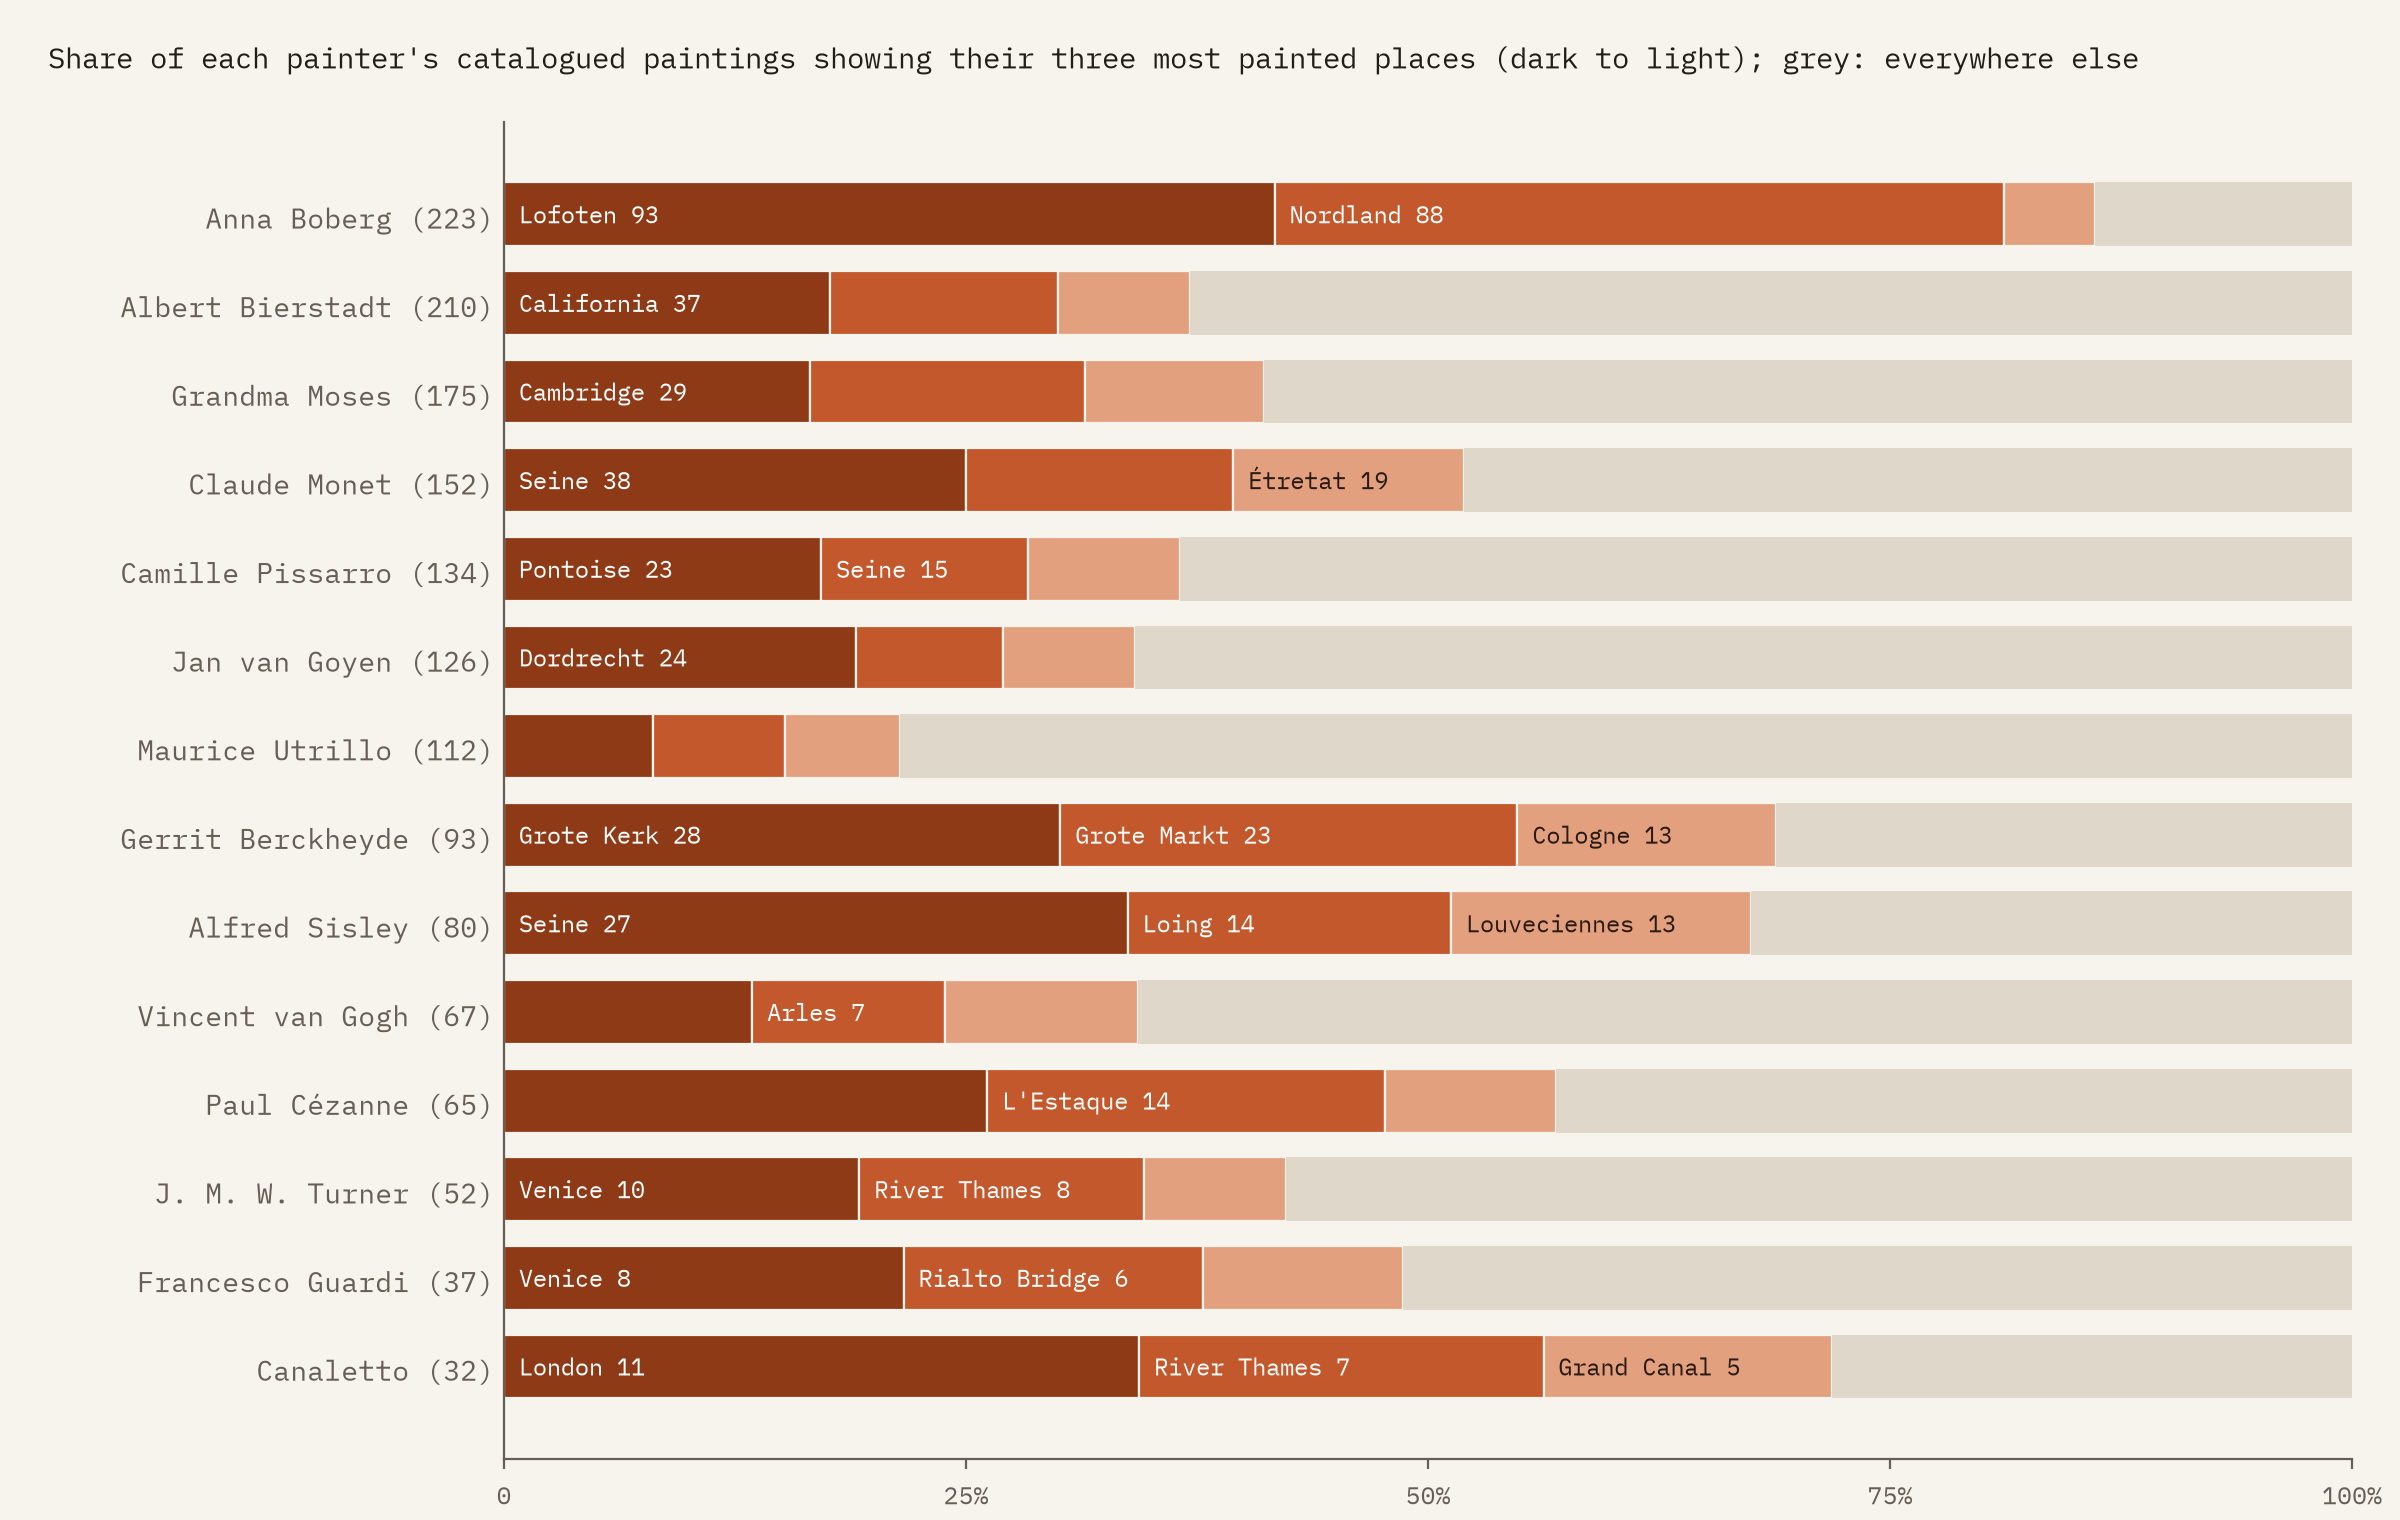
\includegraphics[width=\textwidth]{f_painters.png}\caption{Share of each painter's catalogued paintings showing their three most painted places.}\label{fig:painters}\end{figure}
\begin{figure}[tbp]\centering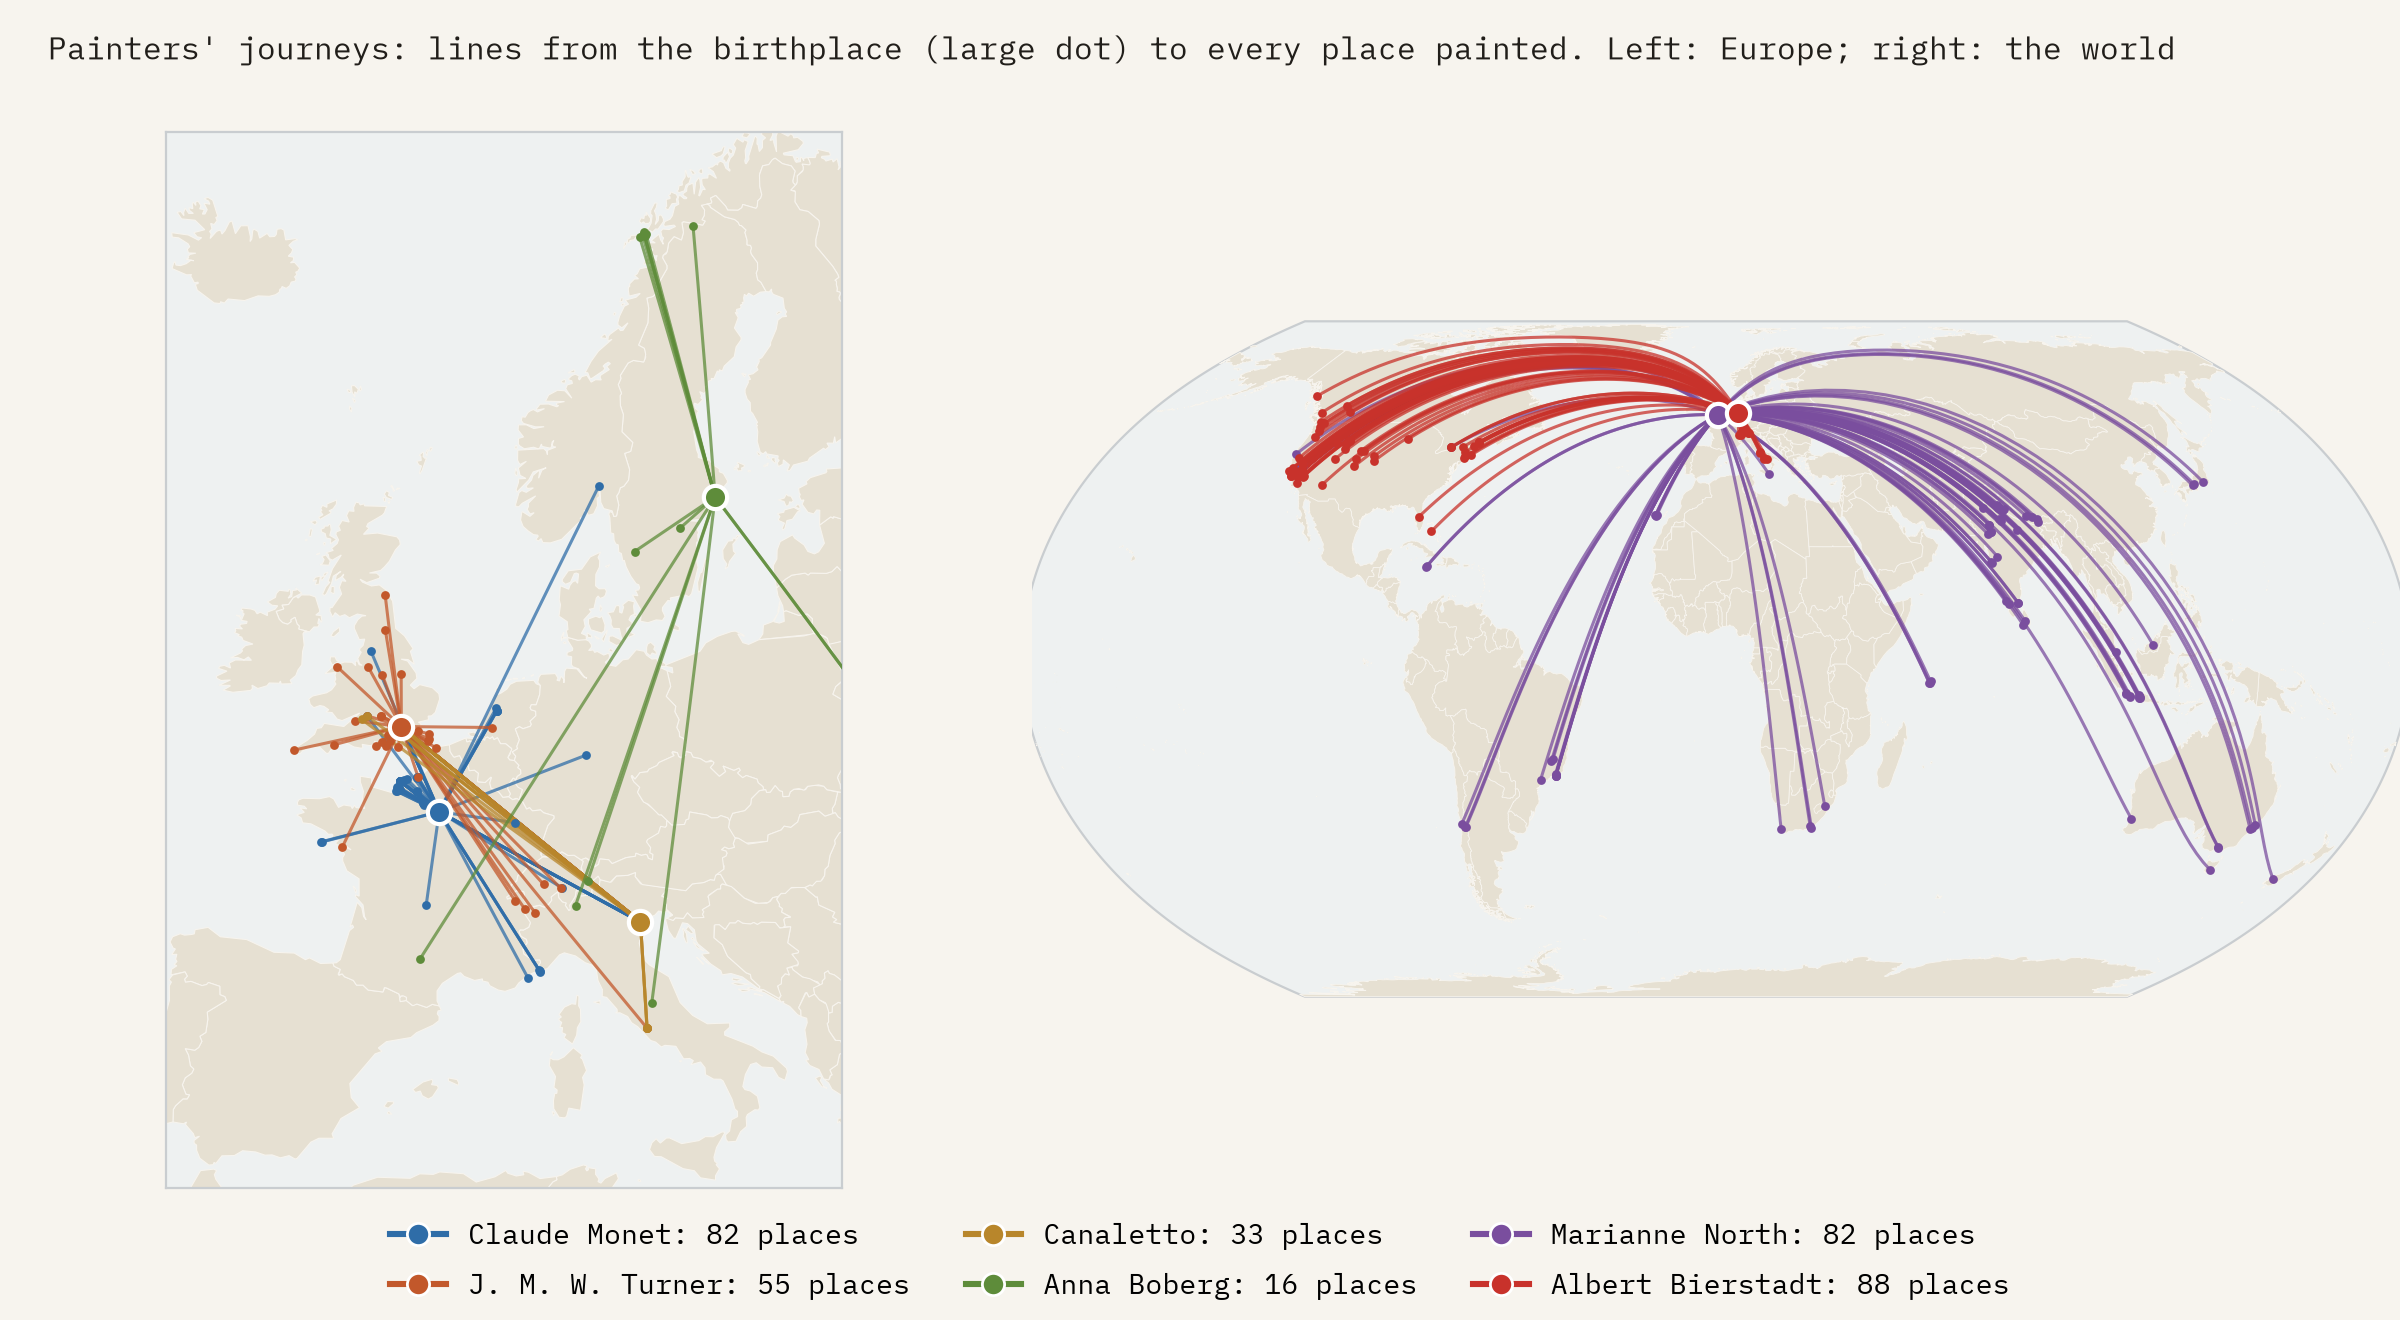
\includegraphics[width=\textwidth]{f_journeys.png}\caption{Lines from the birthplace to every painted place for six painters.}\label{fig:journeys}\end{figure}

\subsection{Distance from home}
Distances are available for 7,183 paintings (84\%) by 2,039 painters. The median is 231 km; 13\% are within 10 km of the birthplace, 26\% within 50 km, 26\% beyond 1,000 km and 11\% beyond 5,000 km (Figure~\ref{fig:distance}). The 1600s are the most local period (median 48 km, 51\% within 50 km); the median rises to 204 km in the 1700s and 331 km in the 1800s, when 31\% of paintings lie more than 1,000 km from the birthplace, and falls to 232 km after 1900. By country of birth (Table~\ref{tab:countries}), painters born in the Netherlands are the most local (median 47 km) and painters born in the United Kingdom (407 km) and Germany (887 km) the most distant among the large groups; British born painters' distant paintings most often show the United States and Italy. Among painters with at least 5 measurable paintings, the largest medians belong to painters who worked at the antipodes of their birthplace, and to Marianne North (94 paintings, median 8,467 km, 20 countries). Some long distances record emigration rather than travel: Bierstadt (8,140 km) and Pissarro (6,815 km) were born in Germany and on St Thomas.

\begin{figure}[tbp]\centering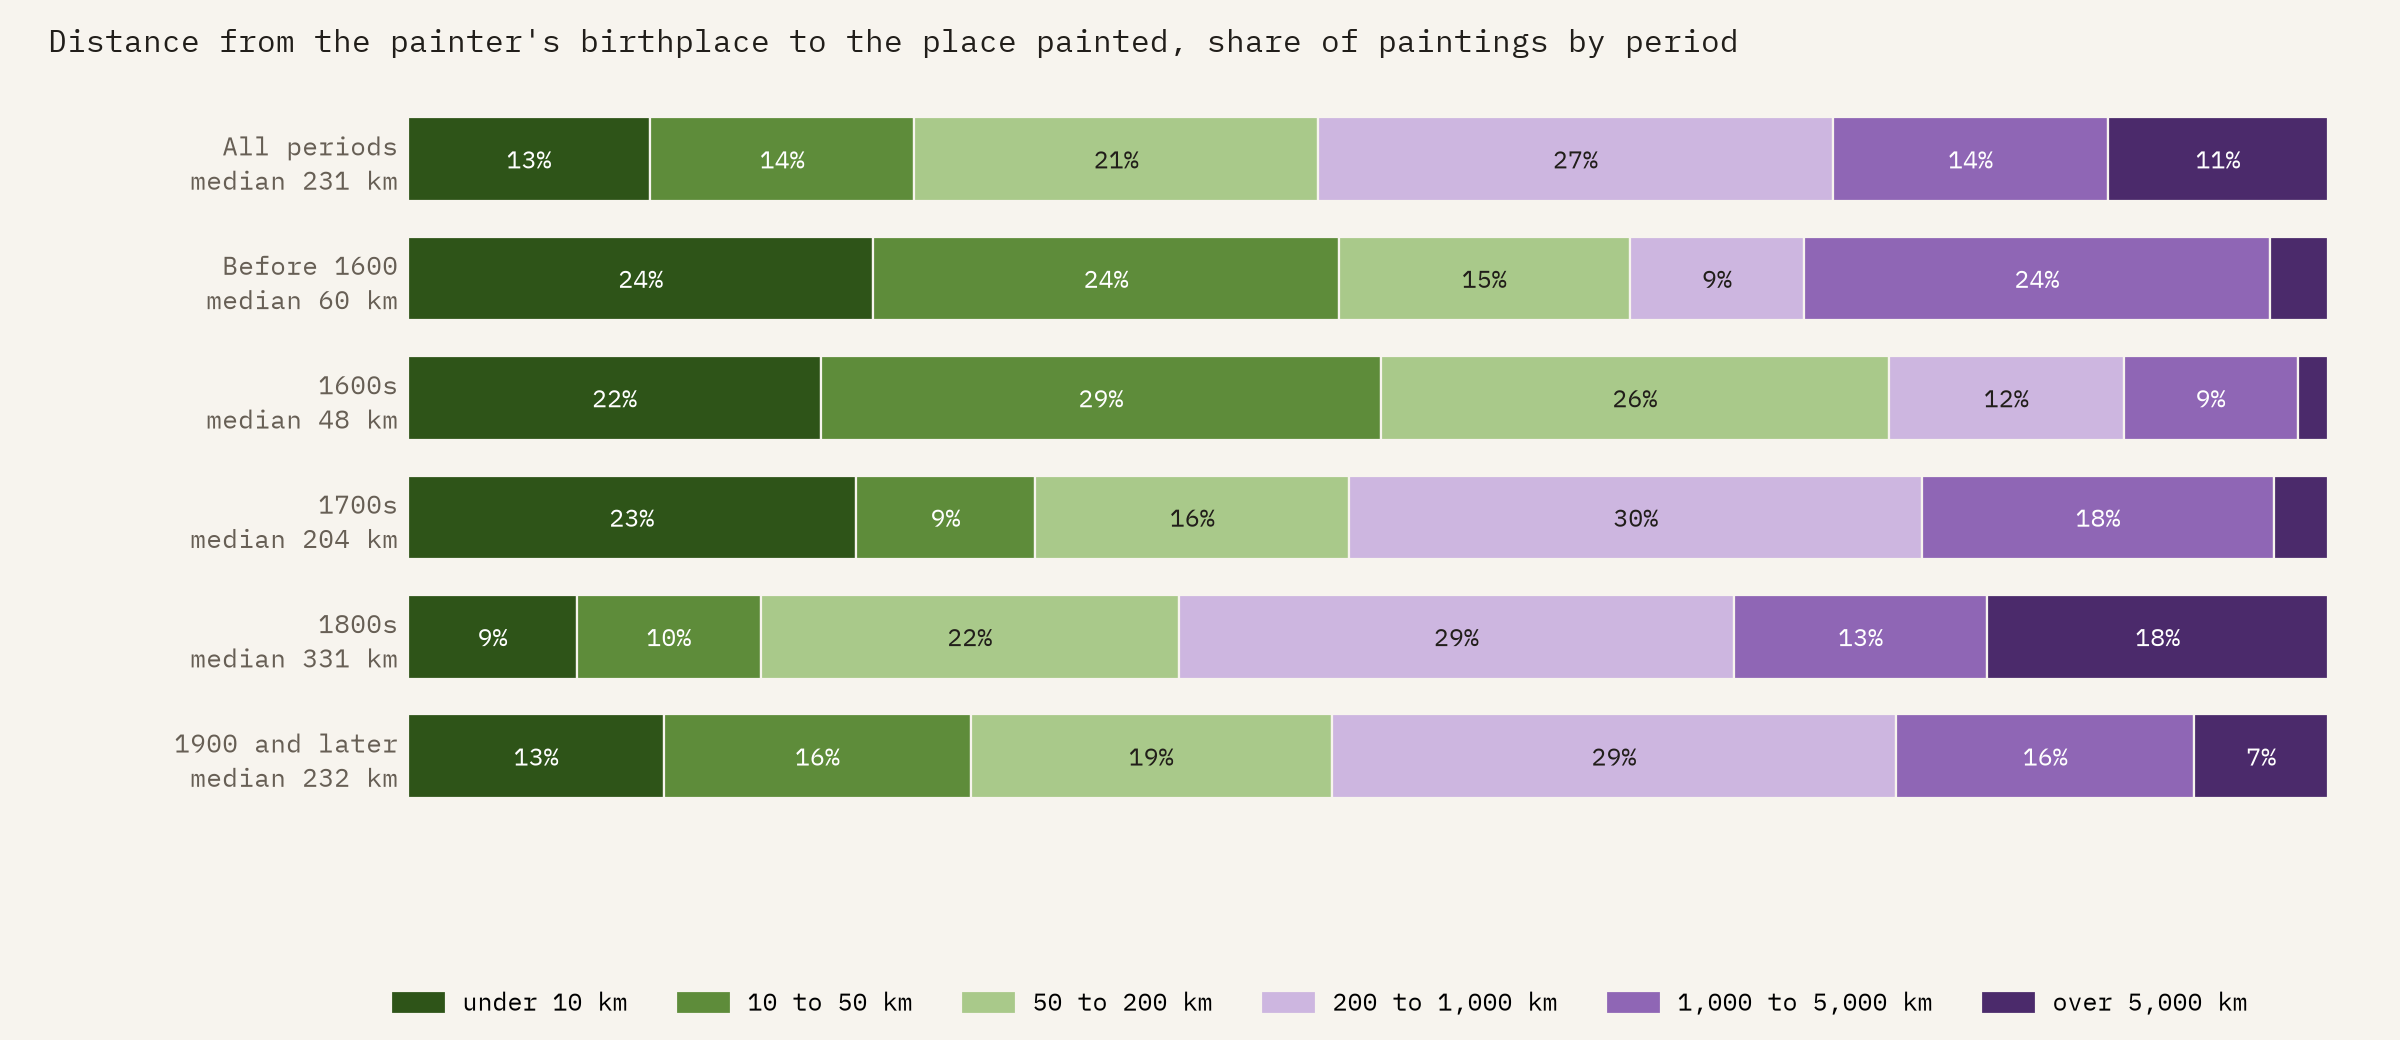
\includegraphics[width=\textwidth]{f_distance.png}\caption{Distance from the painter's birthplace to the place painted, by period.}\label{fig:distance}\end{figure}

\begin{table}[tbp]\centering\footnotesize\caption{Distance from birthplace by the painter's country of birth (today's borders; at least 80 paintings and 20 painters).}\label{tab:countries}\begin{tabular}{lrrrrr}\toprule Born in & Paintings & Painters & Median km & Within 50 km & Over 1,000 km\\\midrule
France & 1,706 & 456 & 175 & 30\% & 11\%\\
Netherlands & 1,091 & 243 & 47 & 51\% & 8\%\\
United Kingdom & 743 & 256 & 407 & 10\% & 44\%\\
United States & 681 & 112 & 279 & 27\% & 28\%\\
Germany & 497 & 144 & 887 & 12\% & 48\%\\
Norway & 393 & 73 & 258 & 13\% & 24\%\\
Sweden & 387 & 92 & 1,004 & 16\% & 52\%\\
Italy & 244 & 91 & 111 & 44\% & 19\%\\
Denmark & 232 & 70 & 156 & 23\% & 12\%\\
Belgium & 208 & 118 & 104 & 39\% & 21\%\\
Spain & 135 & 62 & 383 & 26\% & 18\%\\
Russia & 132 & 38 & 1,035 & 11\% & 61\%\\
Poland & 97 & 52 & 341 & 13\% & 23\%\\
\bottomrule\end{tabular}\end{table}

\subsection{Through the centuries}
The country of the depicted places shifts over time (Figure~\ref{fig:periods}). The Netherlands account for 62\% of 1600s paintings and 3\% of 1800s ones; Italy for 37\% of 1700s paintings, with the United Kingdom second at 23\%; France for 27\% of 1800s and 32\% of later paintings, and the United States for 14\% of 1800s paintings. Norway rises from about 1\% before 1800 to 9\% after 1900, or 6\% without Anna Boberg.

\begin{figure}[tbp]\centering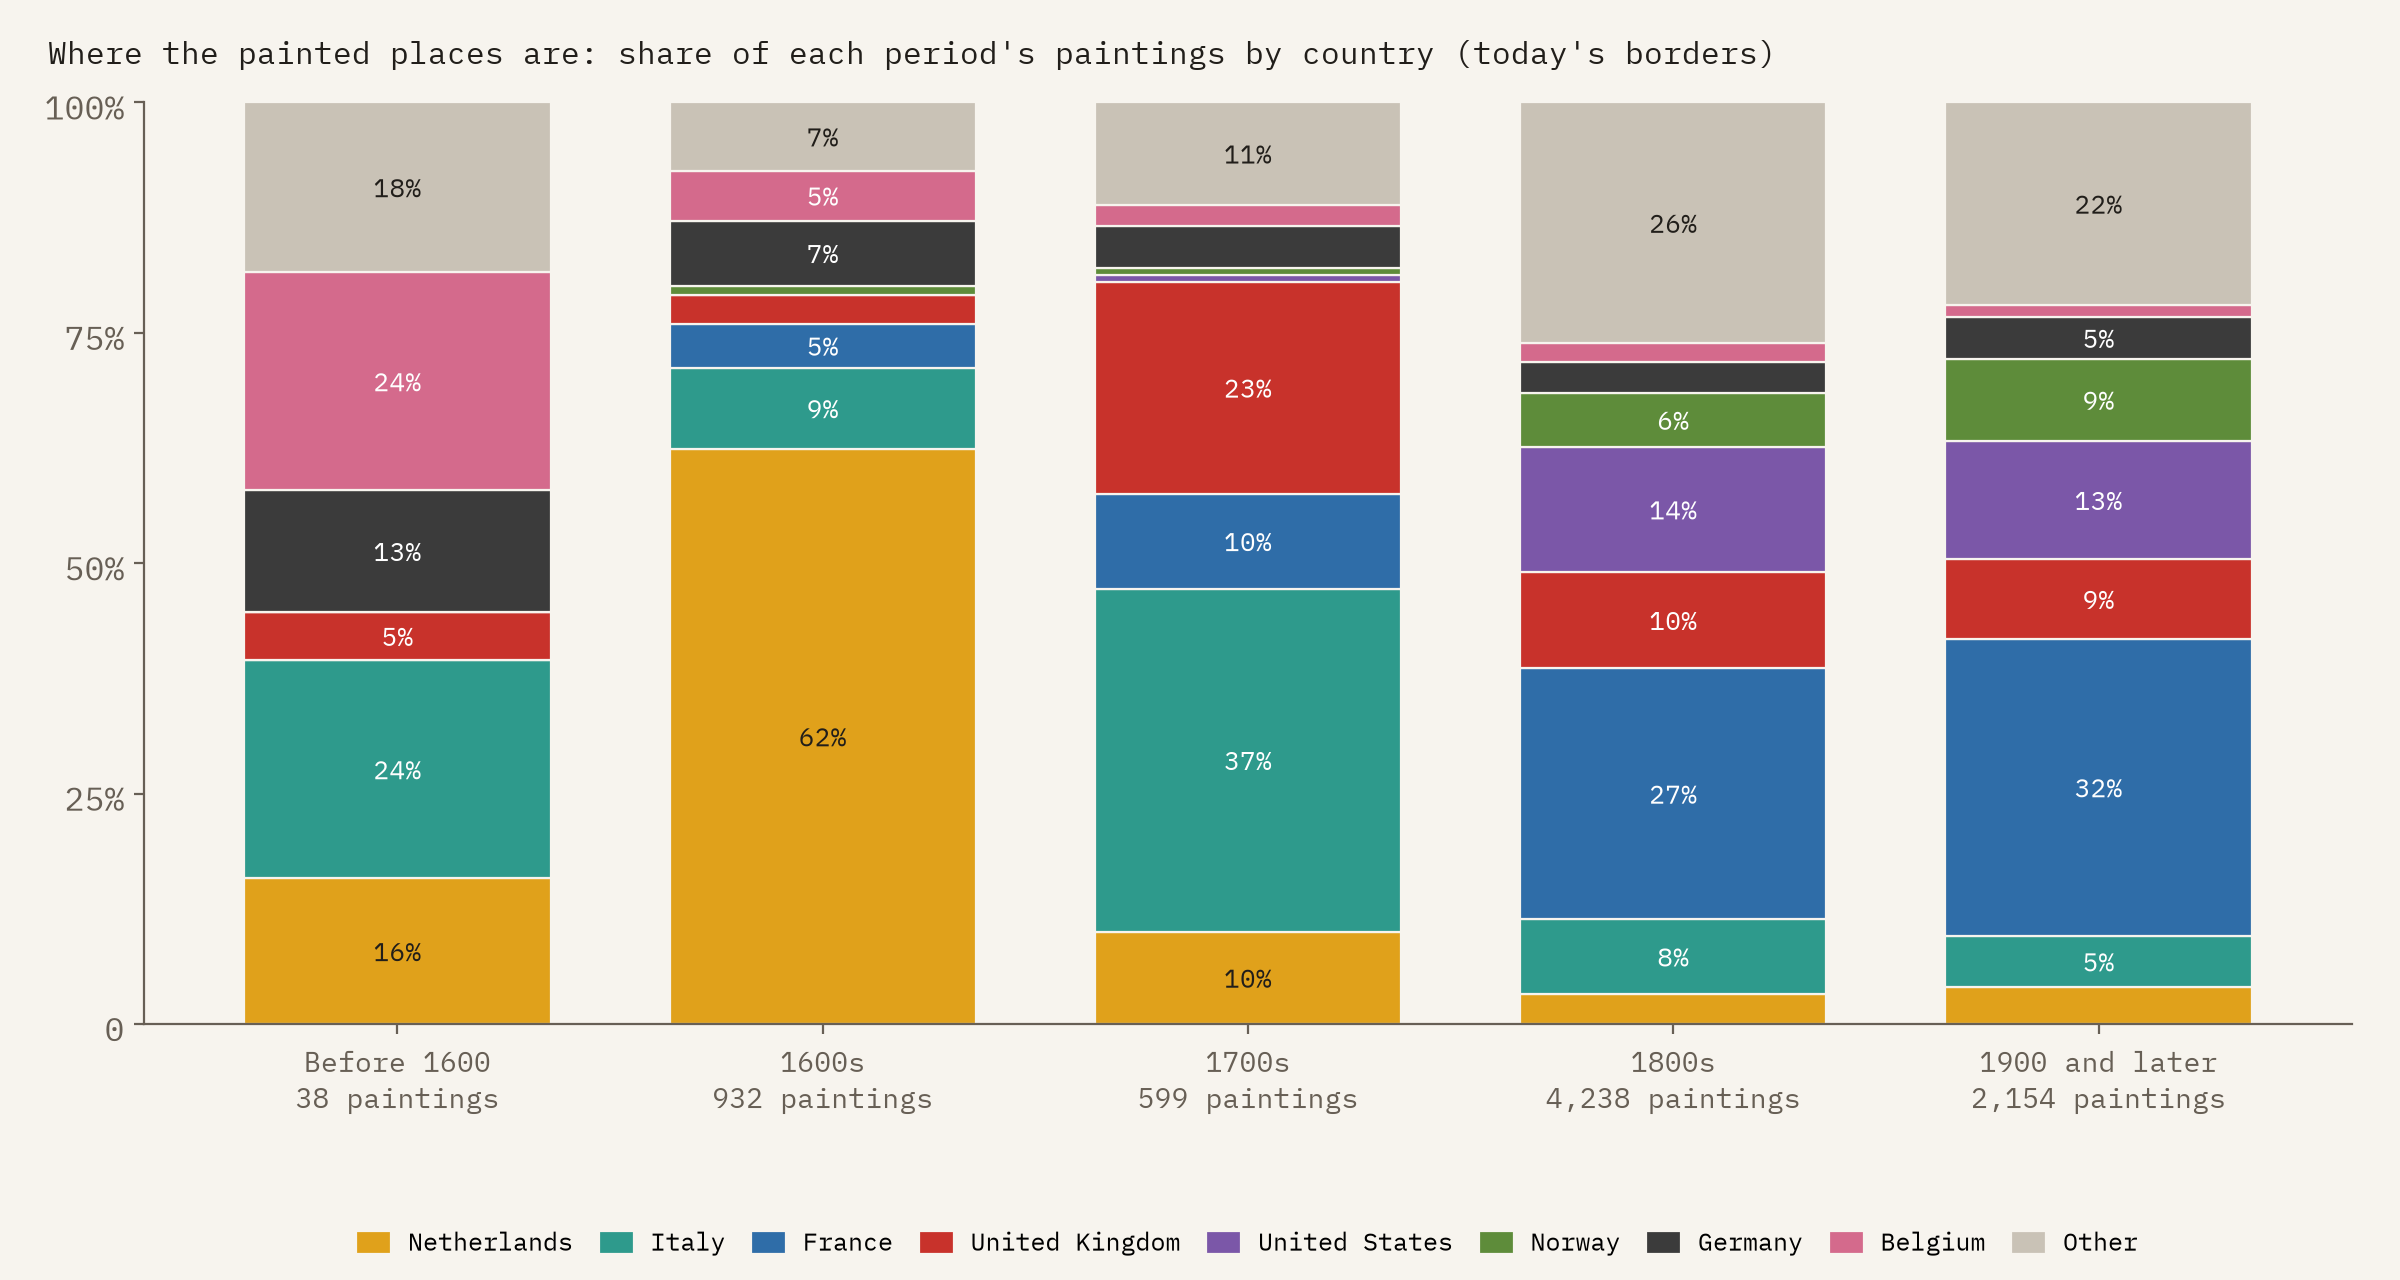
\includegraphics[width=\textwidth]{f_periods.png}\caption{Share of each period's paintings by the country of the depicted place.}\label{fig:periods}\end{figure}

\subsection{Coverage}
The paintings are linked to 1,019 collections; 15\% have none recorded. The largest, Sweden's Nationalmuseum, holds 566 (6.6\%), 222 of them by Anna Boberg, which places Lofoten and Nordland third and fifth among all places. The ten largest collections hold 30\% of paintings and half of all collection links point to 37 collections (3.6\%); 488 collections have one painting (Figure~\ref{fig:collections}, Table~\ref{tab:colls}). Of the 20 most painted places, 4 owe half or more of their paintings to one painter and 4 to one collection. Only 18\% of paintings have a Wikipedia article, 83\% have an image, and 80\% show places in Europe, 12\% in North America and 8\% elsewhere.

\begin{figure}[tbp]\centering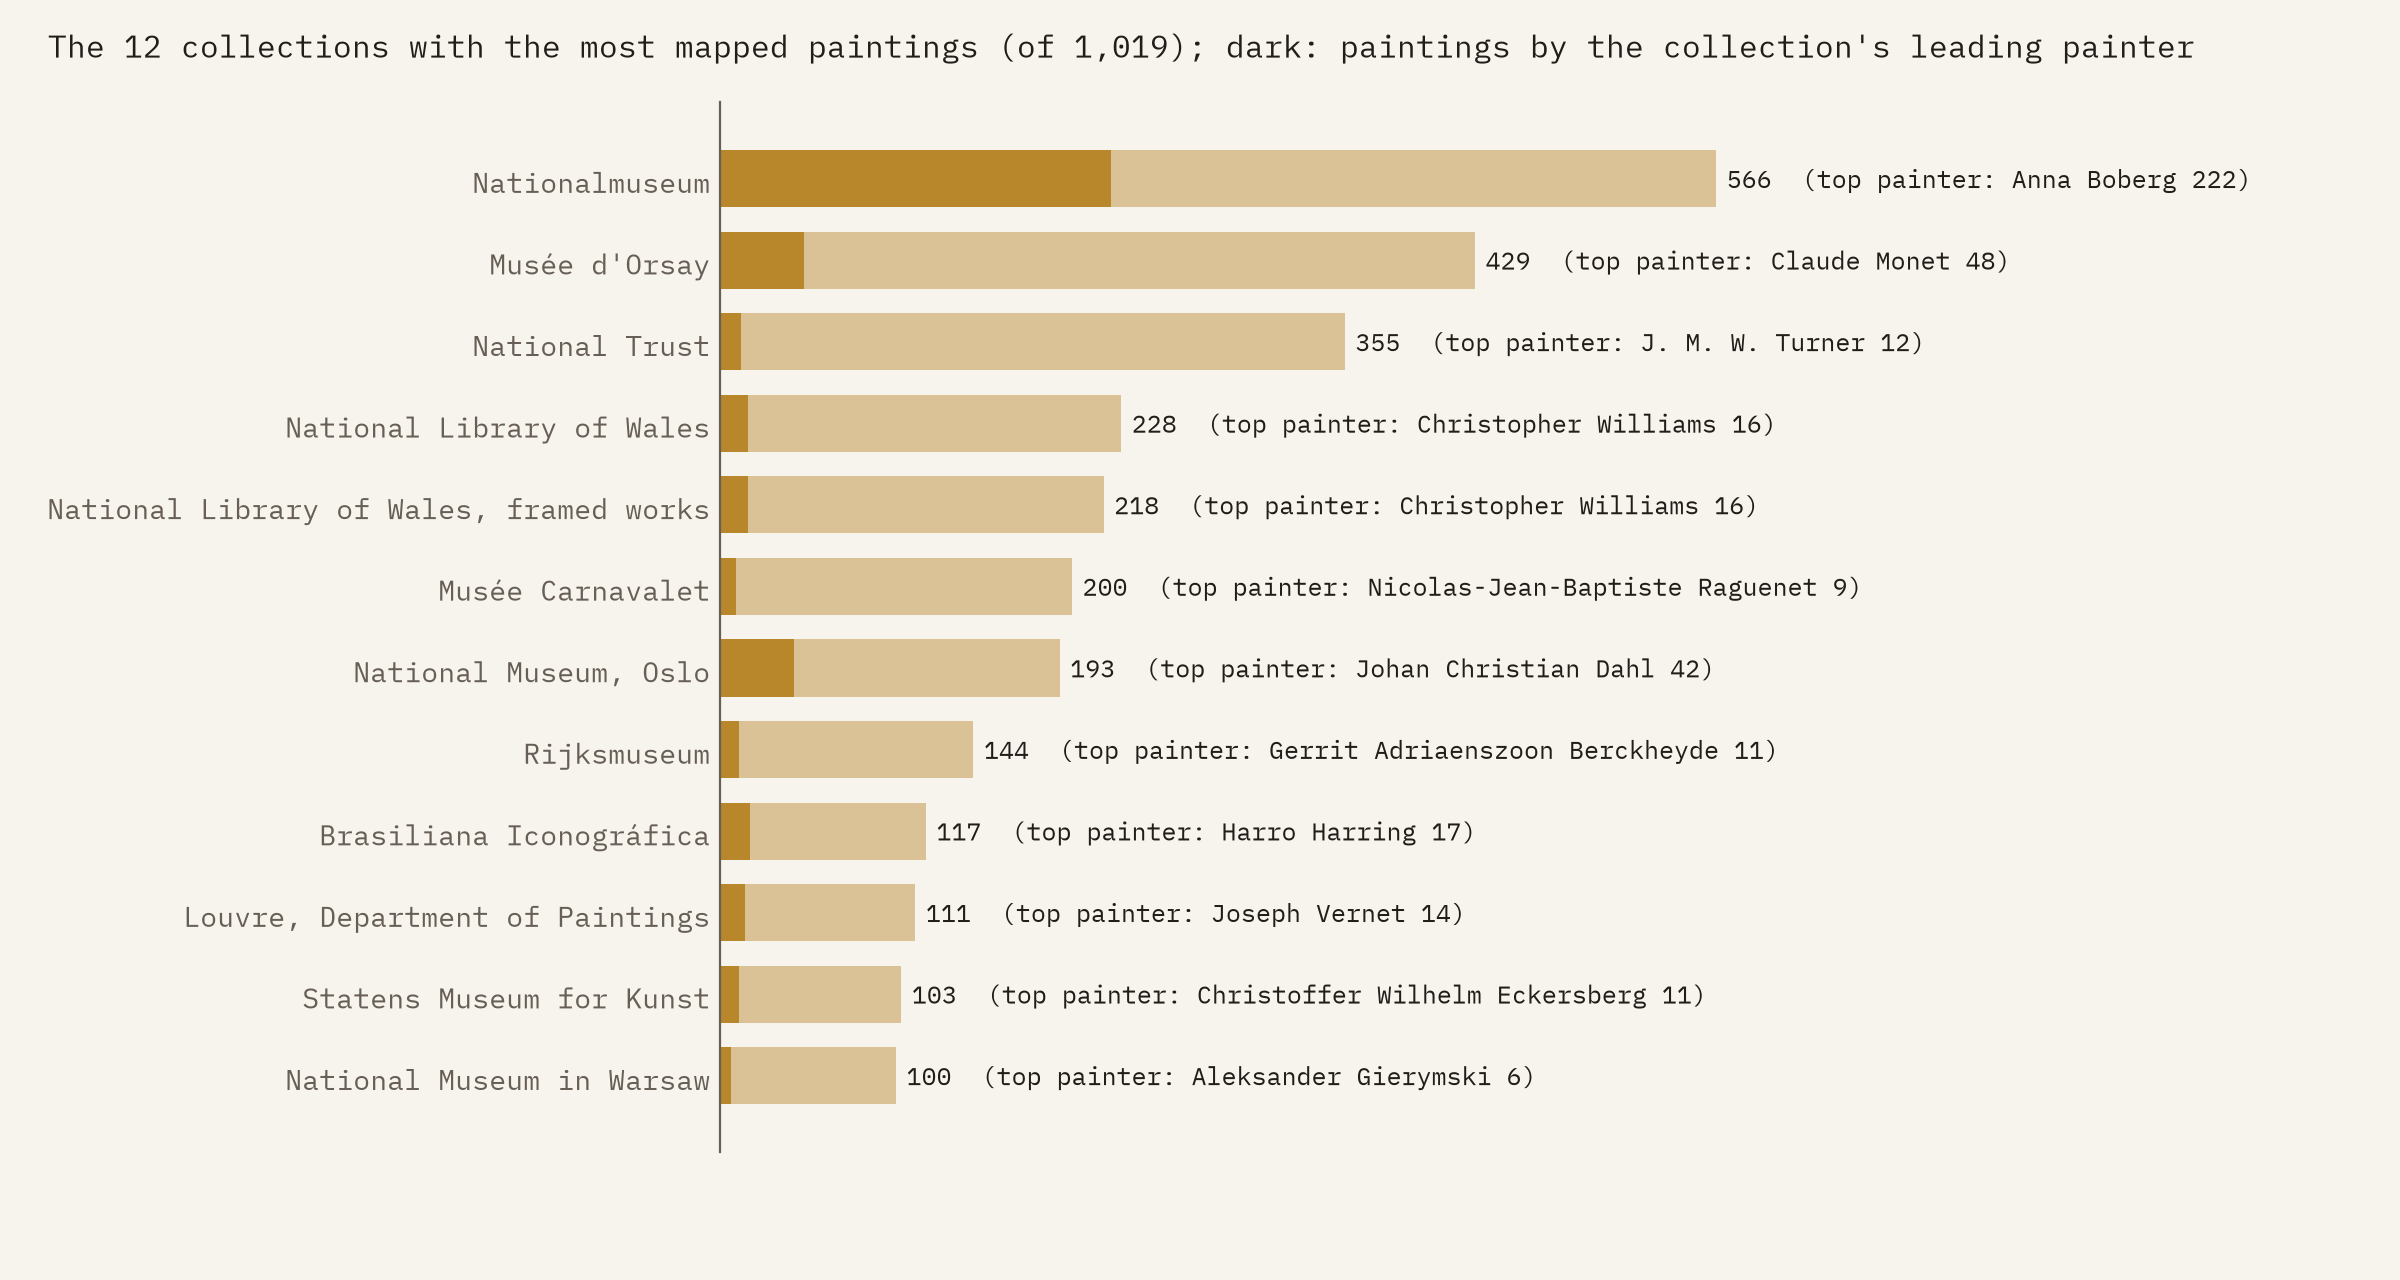
\includegraphics[width=\textwidth]{f_collections.png}\caption{The 12 collections with the most mapped paintings; dark segments are the collection's leading painter.}\label{fig:collections}\end{figure}

\begin{table}[tbp]\centering\footnotesize\setlength{\tabcolsep}{4pt}\caption{The 15 collections with the most mapped paintings.}\label{tab:colls}\begin{tabular}{p{4.6cm}rrp{4.2cm}l}\toprule Collection & Paintings & Share & Leading painter & Most painted place\\\midrule
Nationalmuseum & 566 & 6.6\% & Anna Boberg (222) & Lofoten (93)\\
Musée d'Orsay & 429 & 5.0\% & Claude Monet (48) & Seine (73)\\
National Trust & 355 & 4.2\% & J. M. W. Turner (12) & Windsor Castle (50)\\
National Library of Wales & 228 & 2.7\% & Christopher Williams (16) & Snowdon (10)\\
National Library of Wales Framed works of art collection & 218 & 2.5\% & Christopher Williams (16) & Snowdon (10)\\
Musée Carnavalet & 200 & 2.3\% & Nicolas-Jean-Baptiste Raguenet (9) & Seine (15)\\
National Museum of Art, Architecture and Design & 193 & 2.3\% & Johan Christian Dahl (42) & Elbe (12)\\
Rijksmuseum & 144 & 1.7\% & Gerrit Adriaenszoon Berckheyde (11) & Dam Square (8)\\
Brasiliana Iconográfica & 117 & 1.4\% & Harro Harring (17) & Rio de Janeiro (68)\\
Department of Paintings of the Louvre & 111 & 1.3\% & Joseph Vernet (14) & Italy (7)\\
Statens Museum for Kunst & 103 & 1.2\% & Christoffer Wilhelm Eckersberg (11) & Øresund (7)\\
National Museum in Warsaw & 100 & 1.2\% & Aleksander Gierymski (6) & Tatra Mountains (7)\\
Amsterdam Museum & 93 & 1.1\% & Gerrit Adriaenszoon Berckheyde (6) & Dam Square (10)\\
Metropolitan Museum of Art & 92 & 1.1\% & Claude Monet (7) & Atlantic Ocean (5)\\
Pinacoteca de São Paulo & 88 & 1.0\% & Miguelzinho Dutra (11) & Rio de Janeiro (46)\\
\bottomrule\end{tabular}\end{table}

\section{Limitations}
First, the data are a catalogue, not a sample: a painting appears only if someone recorded its genre and the specific place it depicts, and a few institutions and painters dominate. Second, Wikidata statements can be wrong or loose (a painting tagged with a whole state or county, a river given as a single point), and I have removed only what is clearly not a place. Third, ``depicts'' does not prove the painter visited the place, and the birthplace is a crude proxy for home: emigrants appear as long distance travellers. Fourth, country assignments use today's borders. Fifth, the hand classification of the 100 most painted places by kind is my judgement. Sixth, only one painting in the set carries a separate ``coordinates of depicted place'' statement (Vermeer's View of Delft, within 1.4 km of its depicted places), so place coordinates cannot be validated at scale.

\section{Conclusion}
In the part of Wikidata that records what landscape paintings show, painters returned again and again to rivers, cities and coasts: the Seine above all, Paris, Venice, the Thames, the Hudson and the Dutch river towns. The catalogue captures a clear historical arc, from the painted home towns of the Dutch seventeenth century through the Italian views of the eighteenth to the French rivers and long journeys of the nineteenth. It also captures, just as clearly, the choices of those who built it: one Swedish museum's catalogue of one painter puts the north of Norway near the top of the world's painted places. Read with that in mind, open catalogue data are a promising and transparent way to study the geography of art.

\section*{Data and code availability}
The interactive map is at \url{https://maps.tristanhotham.com/painted-places/}. Data and code are at \url{https://github.com/Tristan-Hotham/painted-places} and archived with this paper at https://doi.org/10.5281/zenodo.23873007. Wikidata content is CC0. Images are not redistributed; the map links to Wikimedia Commons, where each image keeps its own licence. Derived data and text are released under CC BY 4.0 and code under the MIT licence.

\section*{AI statement}
I wrote the text, with drafting and editing assistance from Claude (Anthropic), which also helped prepare the analysis code. I reviewed and checked all text and results.

\begin{thebibliography}{9}
\bibitem[Bast and Buchhold(2017)]{qlever} Bast, H. and Buchhold, B. (2017) QLever: a query engine for efficient SPARQL+text search. In Proceedings of the 2017 ACM Conference on Information and Knowledge Management, 647 to 656.
\bibitem[Natural Earth(2026)]{naturalearth} Natural Earth (2026) Admin 0 countries, admin 1 states and provinces, land, 1:10m and 1:50m. Public domain. \url{https://www.naturalearthdata.com/}
\bibitem[Vrandečić and Krötzsch(2014)]{wikidata} Vrandečić, D. and Krötzsch, M. (2014) Wikidata: a free collaborative knowledgebase. Communications of the ACM 57(10), 78 to 85.
\end{thebibliography}
\end{document}
